%% LyX 1.3 created this file.  For more info, see http://www.lyx.org/.
%% Do not edit unless you really know what you are doing.
\documentclass[english, 12pt]{article}
\usepackage{times}
%\usepackage{algorithm2e}
\usepackage{url}
\usepackage{bbm}
\usepackage[T1]{fontenc}
\usepackage[latin1]{inputenc}
\usepackage{geometry}
\geometry{verbose,letterpaper,tmargin=2.5cm,bmargin=2.5cm,lmargin=2.5cm,rmargin=2.5cm}
\usepackage{rotating}
\usepackage{color}
\usepackage{graphicx}
\usepackage{amsmath, amsthm, amssymb}
\usepackage{setspace}
\usepackage{lineno}
\usepackage{hyperref}
\usepackage{bbm}


%\usepackage{xr}
%\externaldocument{PRS-supp}

\linenumbers
\doublespacing
%\usepackage[authoryear]{natbib}
\usepackage{natbib} \bibpunct{(}{)}{;}{author-year}{}{,} 

%Pour les rajouts
\usepackage{color}
\definecolor{trustcolor}{rgb}{0,0,1}

\usepackage{dsfont}
\usepackage[warn]{textcomp}
\usepackage{adjustbox}
\usepackage{multirow}
\usepackage{graphicx}
\graphicspath{{figures/}}
\DeclareMathOperator*{\argmin}{\arg\!\min}

\let\tabbeg\tabular
\let\tabend\endtabular
\renewenvironment{tabular}{\begin{adjustbox}{max width=\textwidth}\tabbeg}{\tabend\end{adjustbox}}

\makeatletter

%%%%%%%%%%%%%%%%%%%%%%%%%%%%%% LyX specific LaTeX commands.
%% Bold symbol macro for standard LaTeX users
%\newcommand{\boldsymbol}[1]{\mbox{\boldmath $#1$}}

%% Because html converters don't know tabularnewline
\providecommand{\tabularnewline}{\\}

\usepackage{babel}
\makeatother


\begin{document}

\section{Introduction}

In my thesis work, we have been focusing on assessing someone's risk of disease based on DNA mutations data. DNA mutations do not really change over lifetime so that we could, in theory, assess someone's risk of disease at birth. Thus, this could have potentially large implications in disease prevention. As an example, about 12\% of women in the general population will develop breast cancer sometime during their lives \cite[]{desantis2016breast}. By contrast, a recent large study estimated that about 72\% (95\% CI: 65\%-79\%) of women who inherit a harmful BRCA1 mutation and about 69\% (95\% CI: 61\%-77\%) of women who inherit a harmful BRCA2 mutation will develop breast cancer by the age of 80 \cite[]{kuchenbaecker2017risks}. In 2013, Angelina Jolie announced that she had undergone a preventative double mastectomy, because she had a family history of breast cancer and was carrying a harmful BRCA1 mutation. 

In this introduction, [TODO]

\subsection{Context}

Today, clinical risk prediction for common adult-onset diseases often relies on basic demographic characteristics, such as age, gender and ethnicity; basic health parameters and lifestyle factors, such as body mass index, smoking status, alcohol consumption and physical exercise habits; measurement of clinical risk factors proximal to overt disease onset, such as blood pressure levels, blood chemistries or biomarkers indicative of ongoing disease processes; ascertainment of environmental exposures, such as air pollution, heavy metals and other environmental toxins; and family history \cite[]{torkamani2018personal}.
Routine genetic profiling is conspicuously absent from this list, often relegated to use only when testing clarifies individual-level risks in the context of a known family history for some common adult-onset 
diseases \cite[]{torkamani2018personal}.

\subsubsection{Different types of disease and mutations}

Different types of mutations exist (Figure \ref{fig:rare-common}) [PARLER DE DISEASE ARCHITECTURE??].
Like BRCA1 and BRCA2, many other highly penetrant mutations\footnote{most people carrying the mutation will develop the disease} are associated with diseases, and are searchable in an online database \cite[]{hamosh2005online}. Those mutation are often very rare and are either associated with some very rare disease or are explaining only a small proportion of common disease incidence. 
In this work, we focus on common diseases (e.g.\ breast cancer) and try to predict individuals' disease susceptibility based on common variants; the common disease-common variant hypothesis. The hypothesis further suggests that such diseases are likely caused by a large number of common variants, each contributing only a small risk and thereby evading negative evolutionary selection \cite[]{salari2012personalized}.
One common form of variation across human genomes is called a single nucleotide polymorphism (SNP). As indicated by the name, SNPs are single base changes in the DNA. 
Sequencing technologies now exists to genotype hundreds of thousands of variants at once for around \$50 only. Starting with the \cite{wellcome2007genome}, these new sequencing technologies had led to many Genome-Wide Association Studies (GWAS).%, which we talk about in the next section. From these studies, it was found that effects of common variants that are associated with some disease are typically very small.

\begin{figure}[ht]
\centerline{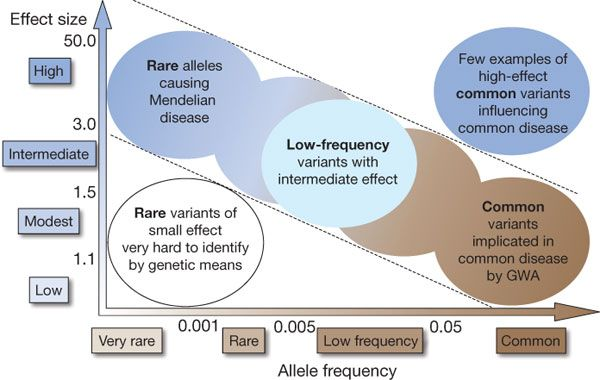
\includegraphics[width=0.7\textwidth]{rare-common.jpg}}
\caption{Feasibility of identifying genetic variants by risk allele frequency and strength of genetic effect (odds ratio). Most emphasis and interest lies
in identifying associations with characteristics shown within diagonal dotted
lines. Source: \cite{manolio2009finding}.}
\label{fig:rare-common}
\end{figure}

\subsubsection{Genome-Wide Association Studies (GWAS)}


\subsubsection{From GWAS to Polygenic Risk Scores (PRS)}

\subsubsection{The differing goals of association testing and risk prediction}


%%%%%%%%%%%%%%%%%%%%%%%%%%%%%%%%%%%%%%%%%%%%%%%%%%%%%%%%%%%%%%%%%%%%%%%%%%%%%%%%

\subsection{Genomic prediction}

\subsubsection{Heritability and missing heritability}

The basic components of disease risk are usually broken down into genetic susceptibility, environmental exposures and lifestyle factors. Thus, all disease incidence cannot be predicted by genetic factors only. 
For a quantitative phenotype, we call heritability ($h^2$) the proportion of phenotypic variation that is attributable to genetic factors \cite[]{visscher2008heritability}. 
So, basically, heritability is the upper bound in terms of prediction power that we can get using a model from genetic variants only. [DONNER DES EXEMPLES]
Methods now enable

\subsubsection{Methods for genomic prediction}

\subsubsection{Objective and main difficulties of the thesis}


\newpage

\bibliographystyle{natbib}
\bibliography{refs}

\end{document}
